\chapter{システムの提案}
\label{chap:system}
本章では、アプリケーションランチャーについての背景を踏まえ、ホットキーを利用した新しいランチャーシステム「Hyper Launcher」を提案する。

\newpage

\section{設計}
既存のホットキー型アプリケーションランチャーに見られる不便を解消するため、

\begin{enumerate}
	\item アプリケーションの登録及びその変更が簡単にできる
	\item 設定が覚えやすい
	\item より強力に操作できる
\end{enumerate}

という3つの目標を実現するランチャーシステム「Hyper Launcher」を設計した。具体的には

\begin{enumerate}
	\item アプリケーションの登録や変更をドラッグアンドドロップによって簡単に行えるようにする
	\item 使用するホットキーの組み合わせを9つに制限し、そこに対してアプリケーションを登録することで、可能な限り認知不可を下げられるようにする
	\item 単一のホットキーの組み合わせに対して複数のアプリケーションを登録できるようにする
\end{enumerate}

というアプリケーションを実装した。

\section{基本操作}
自身の開発環境を考慮し、アプリケーションはmacOS上でデスクトップアプリとして利用できることとする。起動画面を図\ref{fig:hyper-launcher}に示す。
画面は9つのセクションに分けられており、予めそれぞれにホットキーが指定されている。

\begin{figure}[h]
    \begin{center}
       \fbox{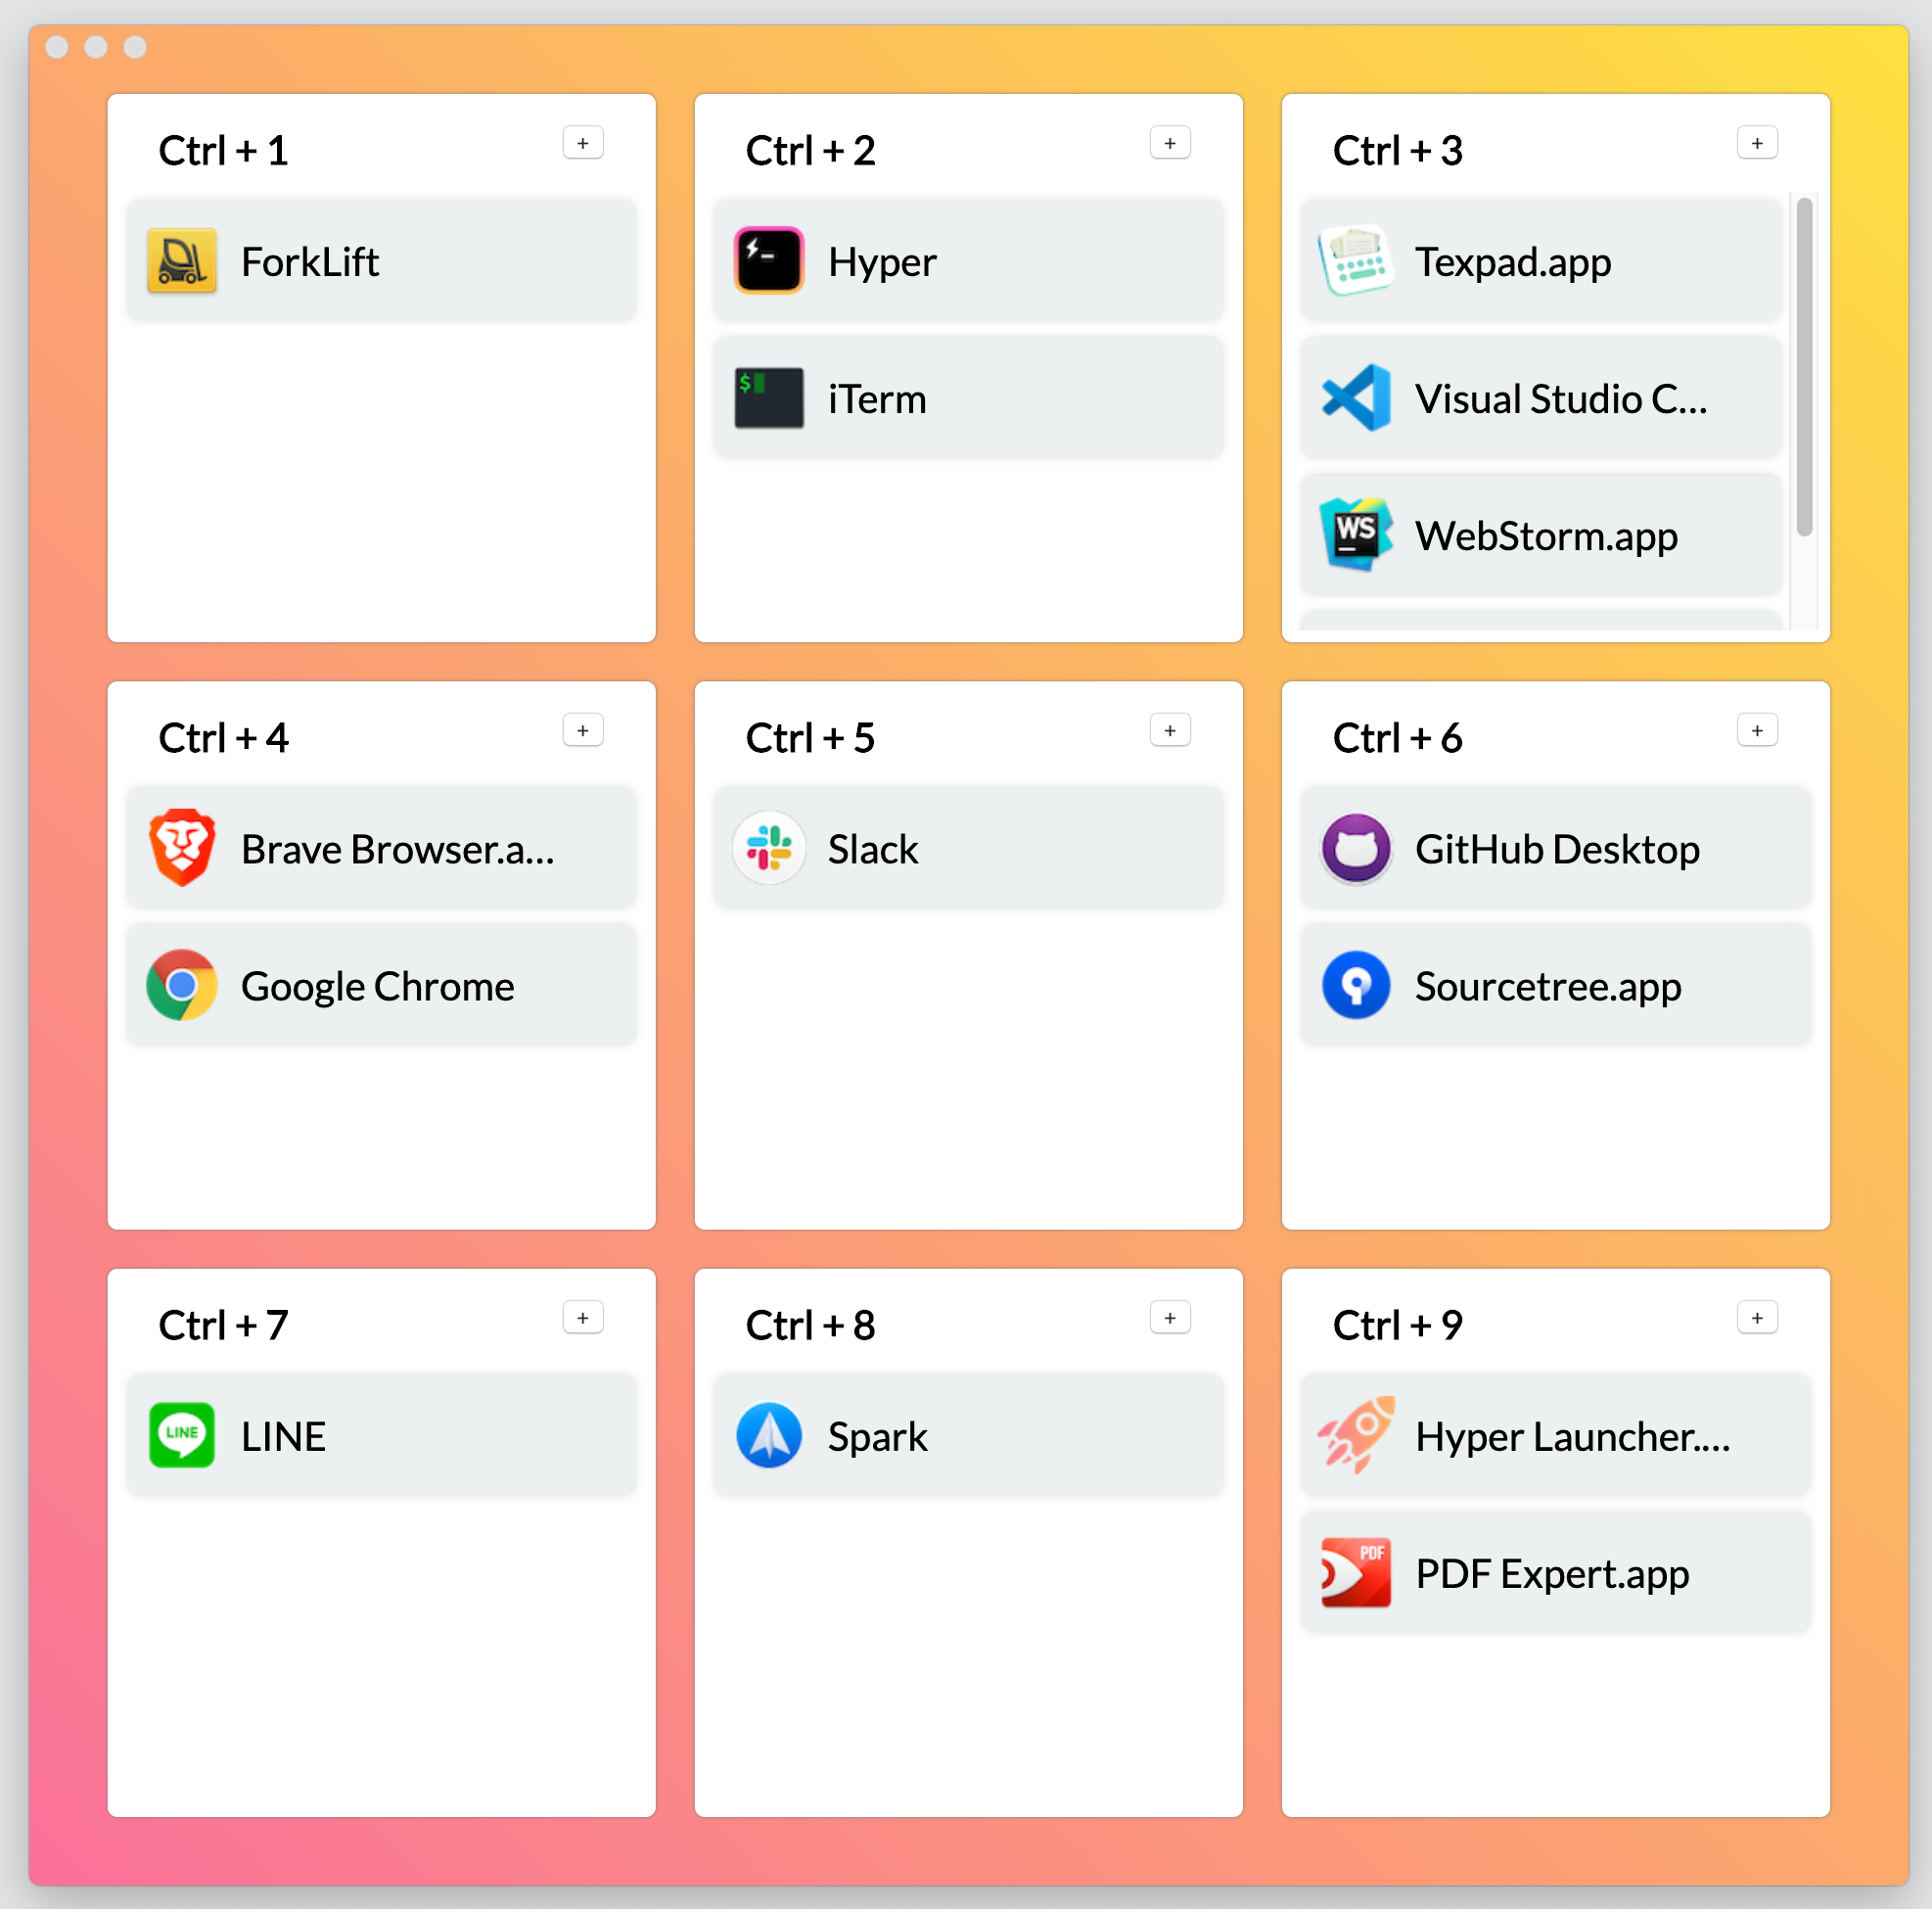
\includegraphics[width=100mm]{images/hyper-launcher}}
    \end{center}
    \caption{Hyper Launcherの起動画面}
    \label{fig:hyper-launcher}
\end{figure}

\subsection{登録と起動}

任意のアプリケーションをそれぞれのセクションにドラッグアンドドロップすることで簡単に登録することができる。また、タイトル横のプラスボタンを押すことでアプリケーション選択画面が出現し、そこからも登録することができる。後は指定されたホットキーを入力するだけでアプリケーションを起動することができる。(図\ref{fig:add1}, \ref{fig:add2})

\begin{figure}[h]
    \begin{center}
       \fbox{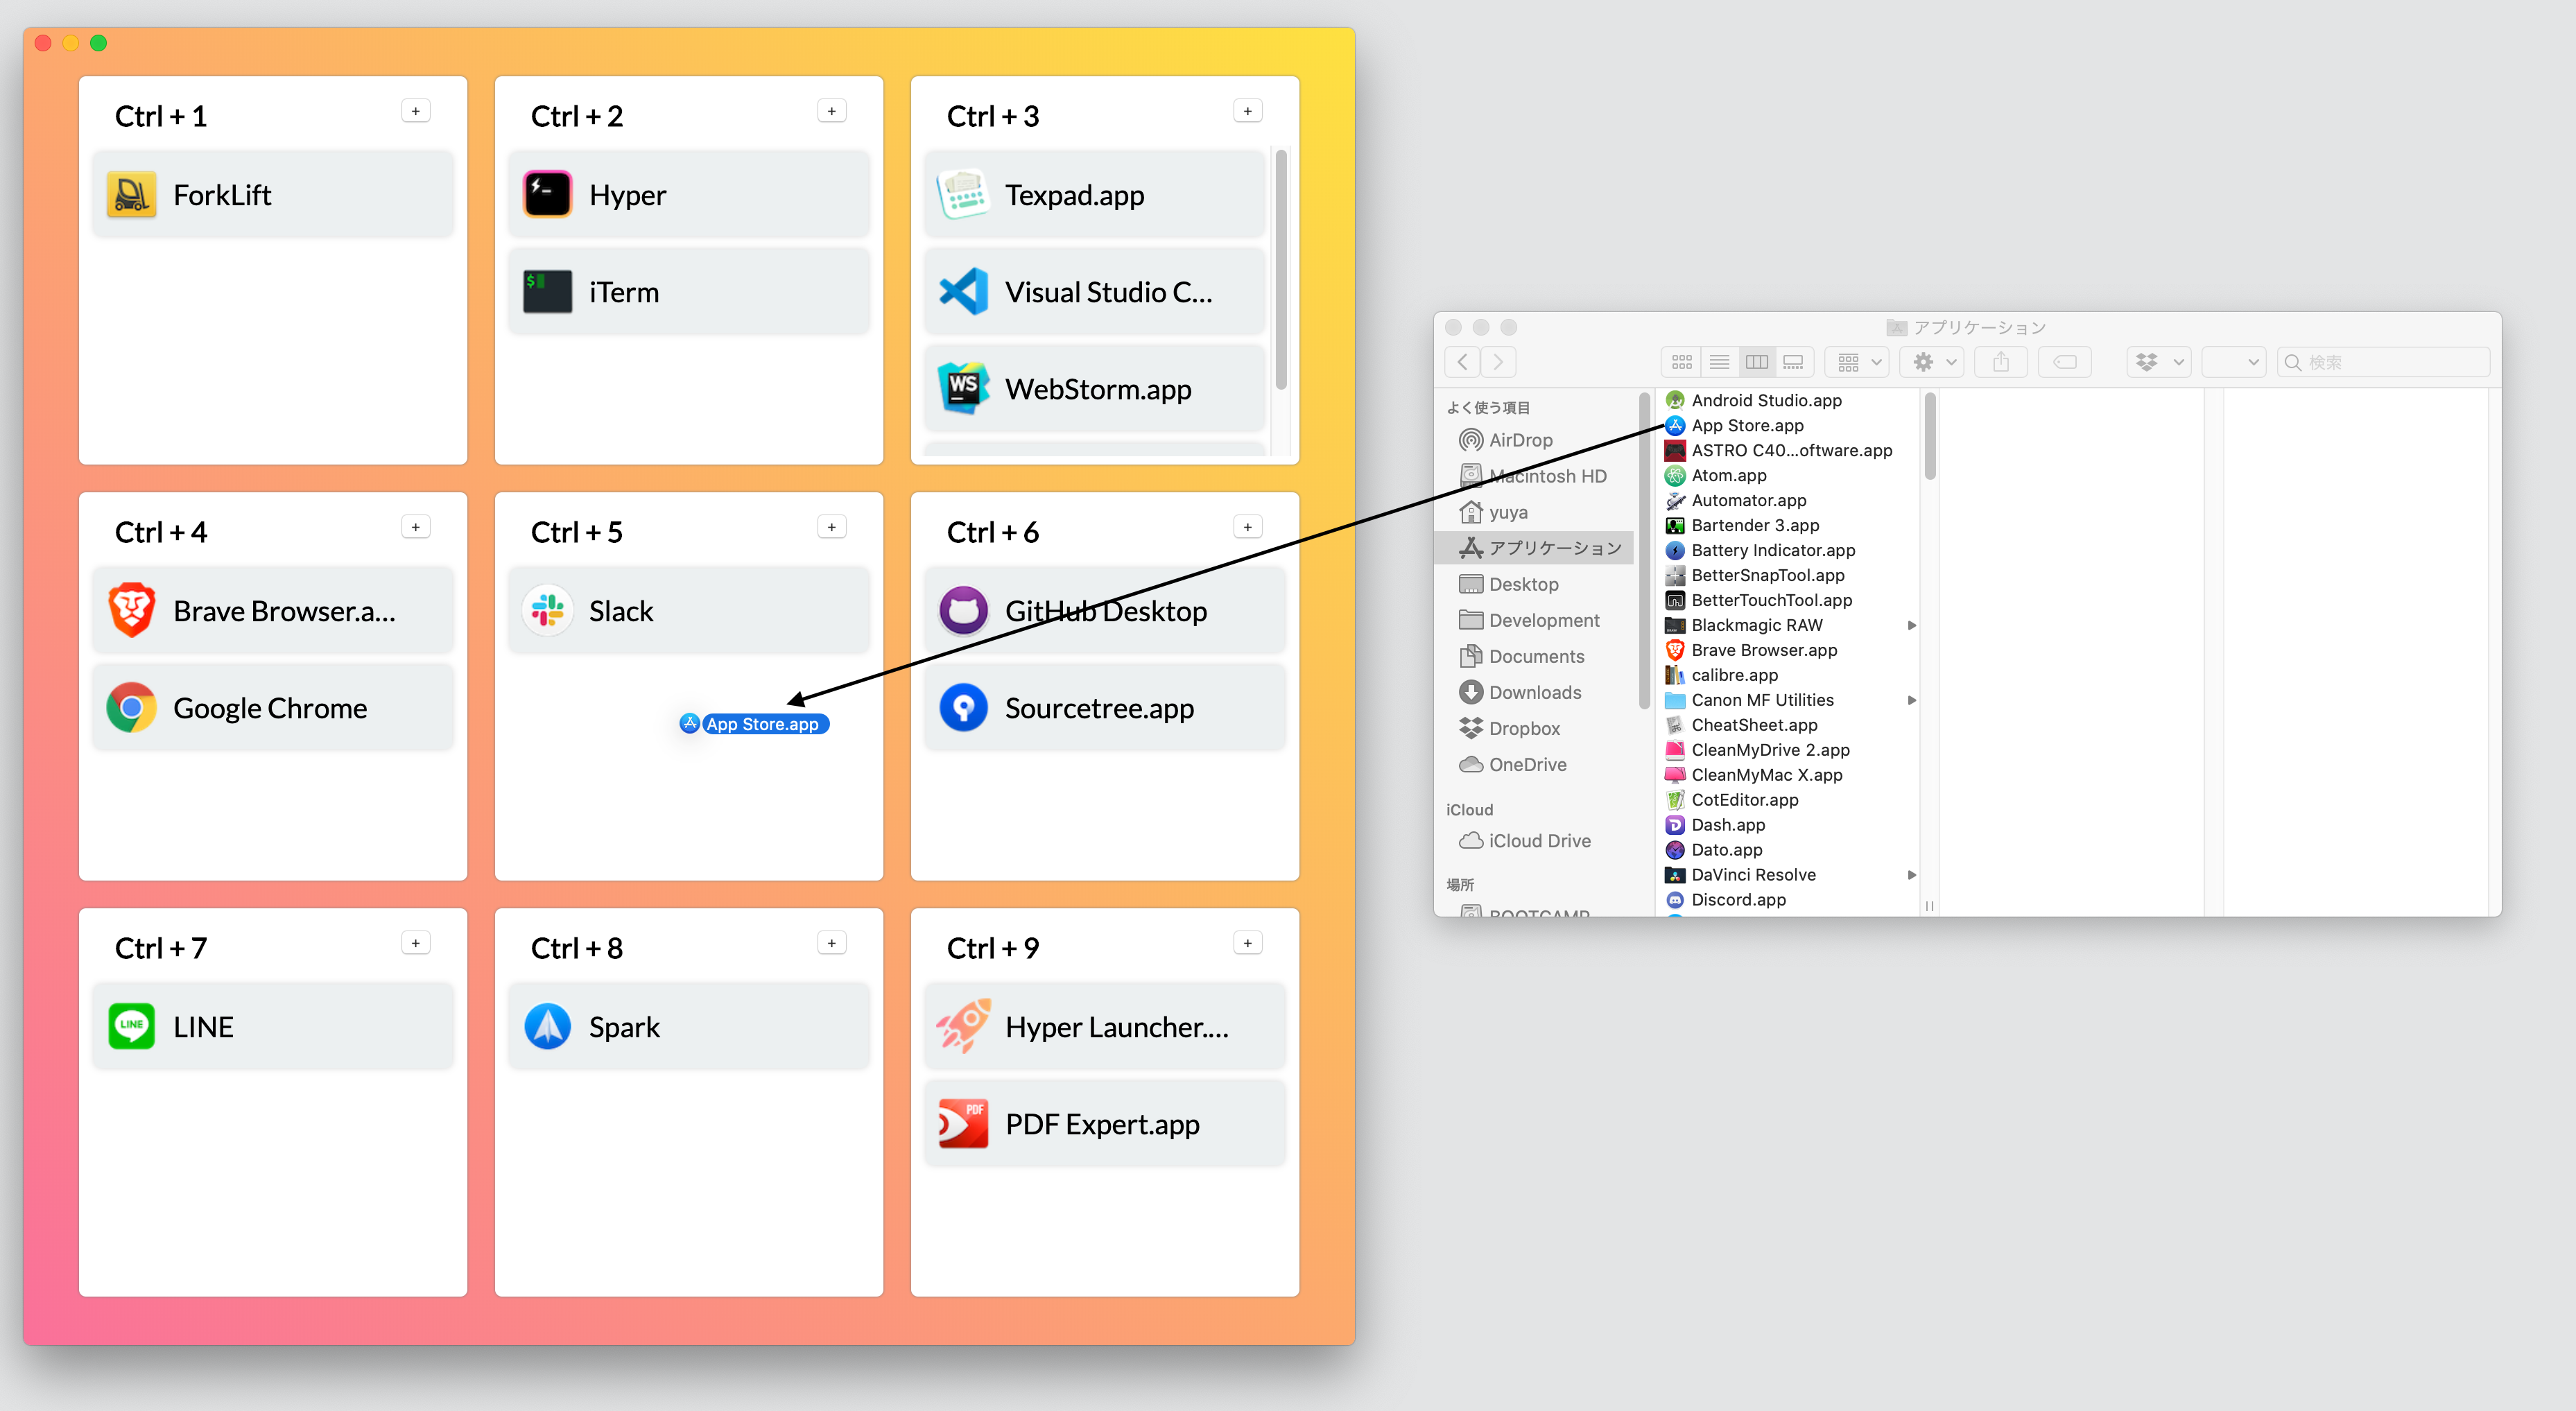
\includegraphics[width=100mm]{images/add1}}
    \end{center}
    \caption{ドラッグアンドドロップによる登録}
    \label{fig:add1}
\end{figure}

\begin{figure}[h]
    \begin{center}
       \fbox{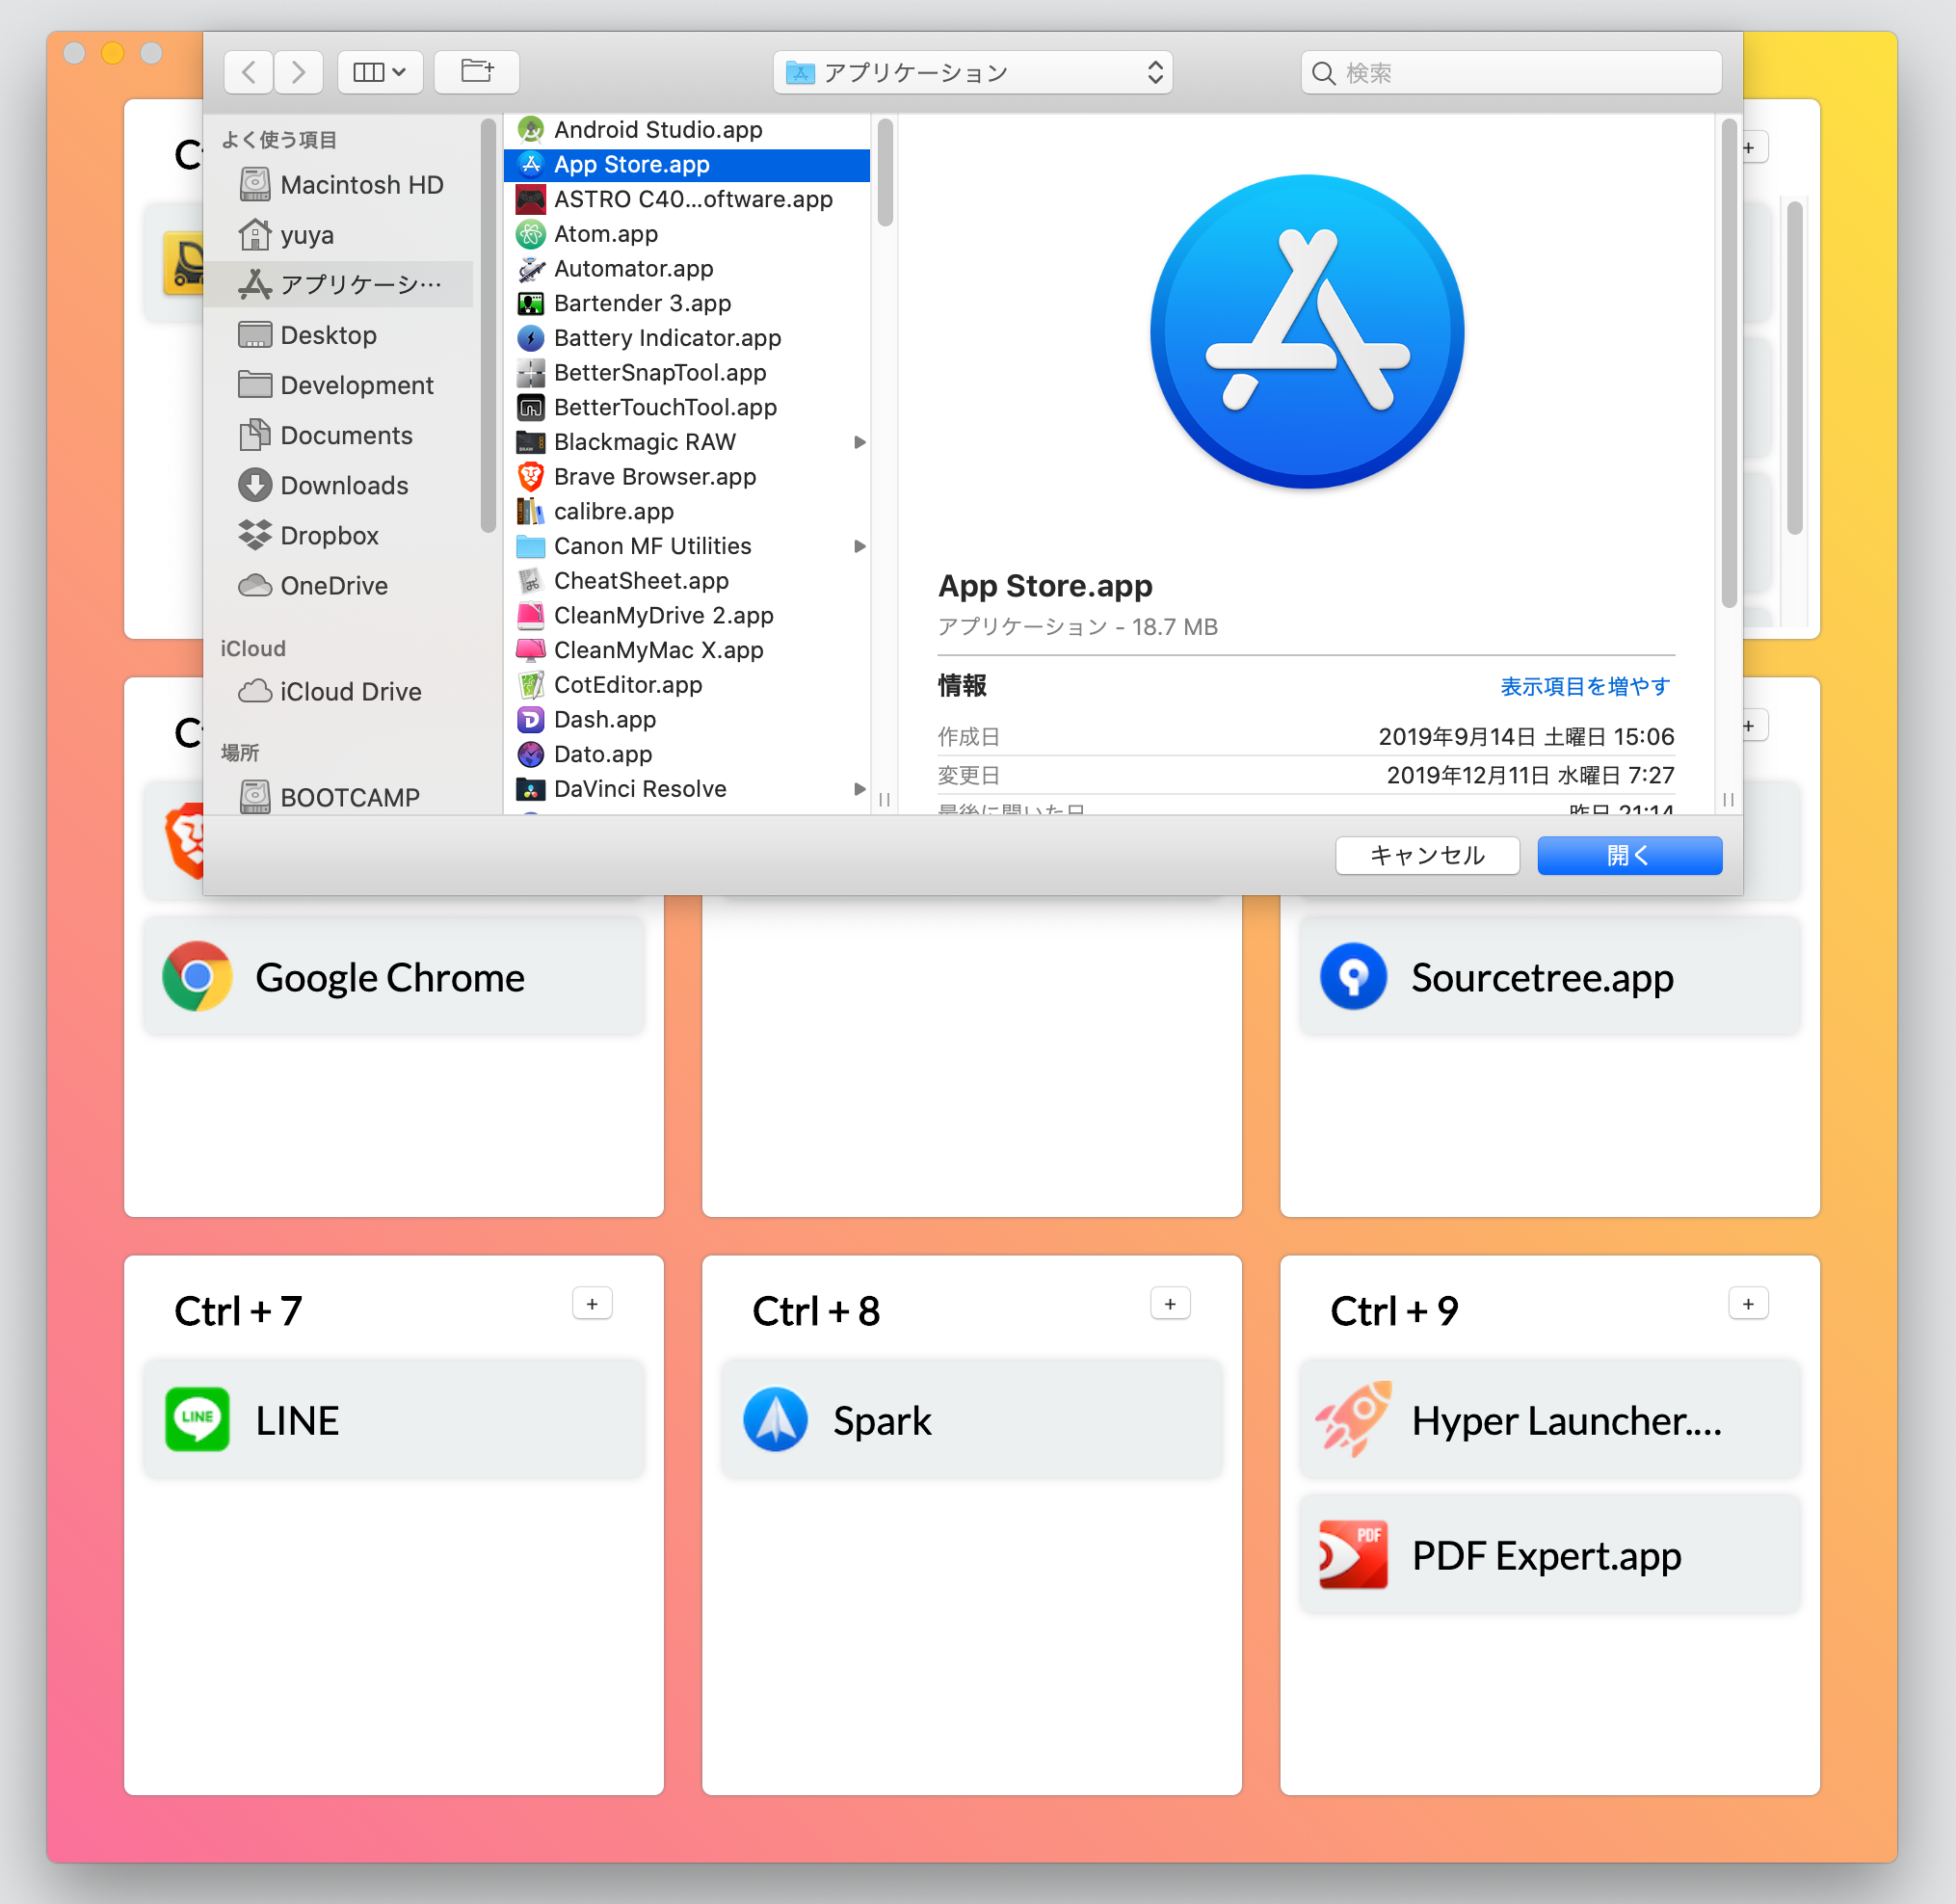
\includegraphics[width=100mm]{images/add2}}
    \end{center}
    \caption{追加ボタンから登録}
    \label{fig:add2}
\end{figure}

\subsection{登録の変更と解除}
アプリケーションに紐付けるホットキーを変更したい時は、対象のアプリケーションを目的のセクションへドラッグアンドドロップするだけで操作が完了する。またアプリケーションにマウスカーソルを乗せた際に右側に表れる削除ボタンを押すことで、登録を解除することができる。(図\ref{fig:change}, \ref{fig:delete})

\begin{figure}[h]
    \begin{center}
       \fbox{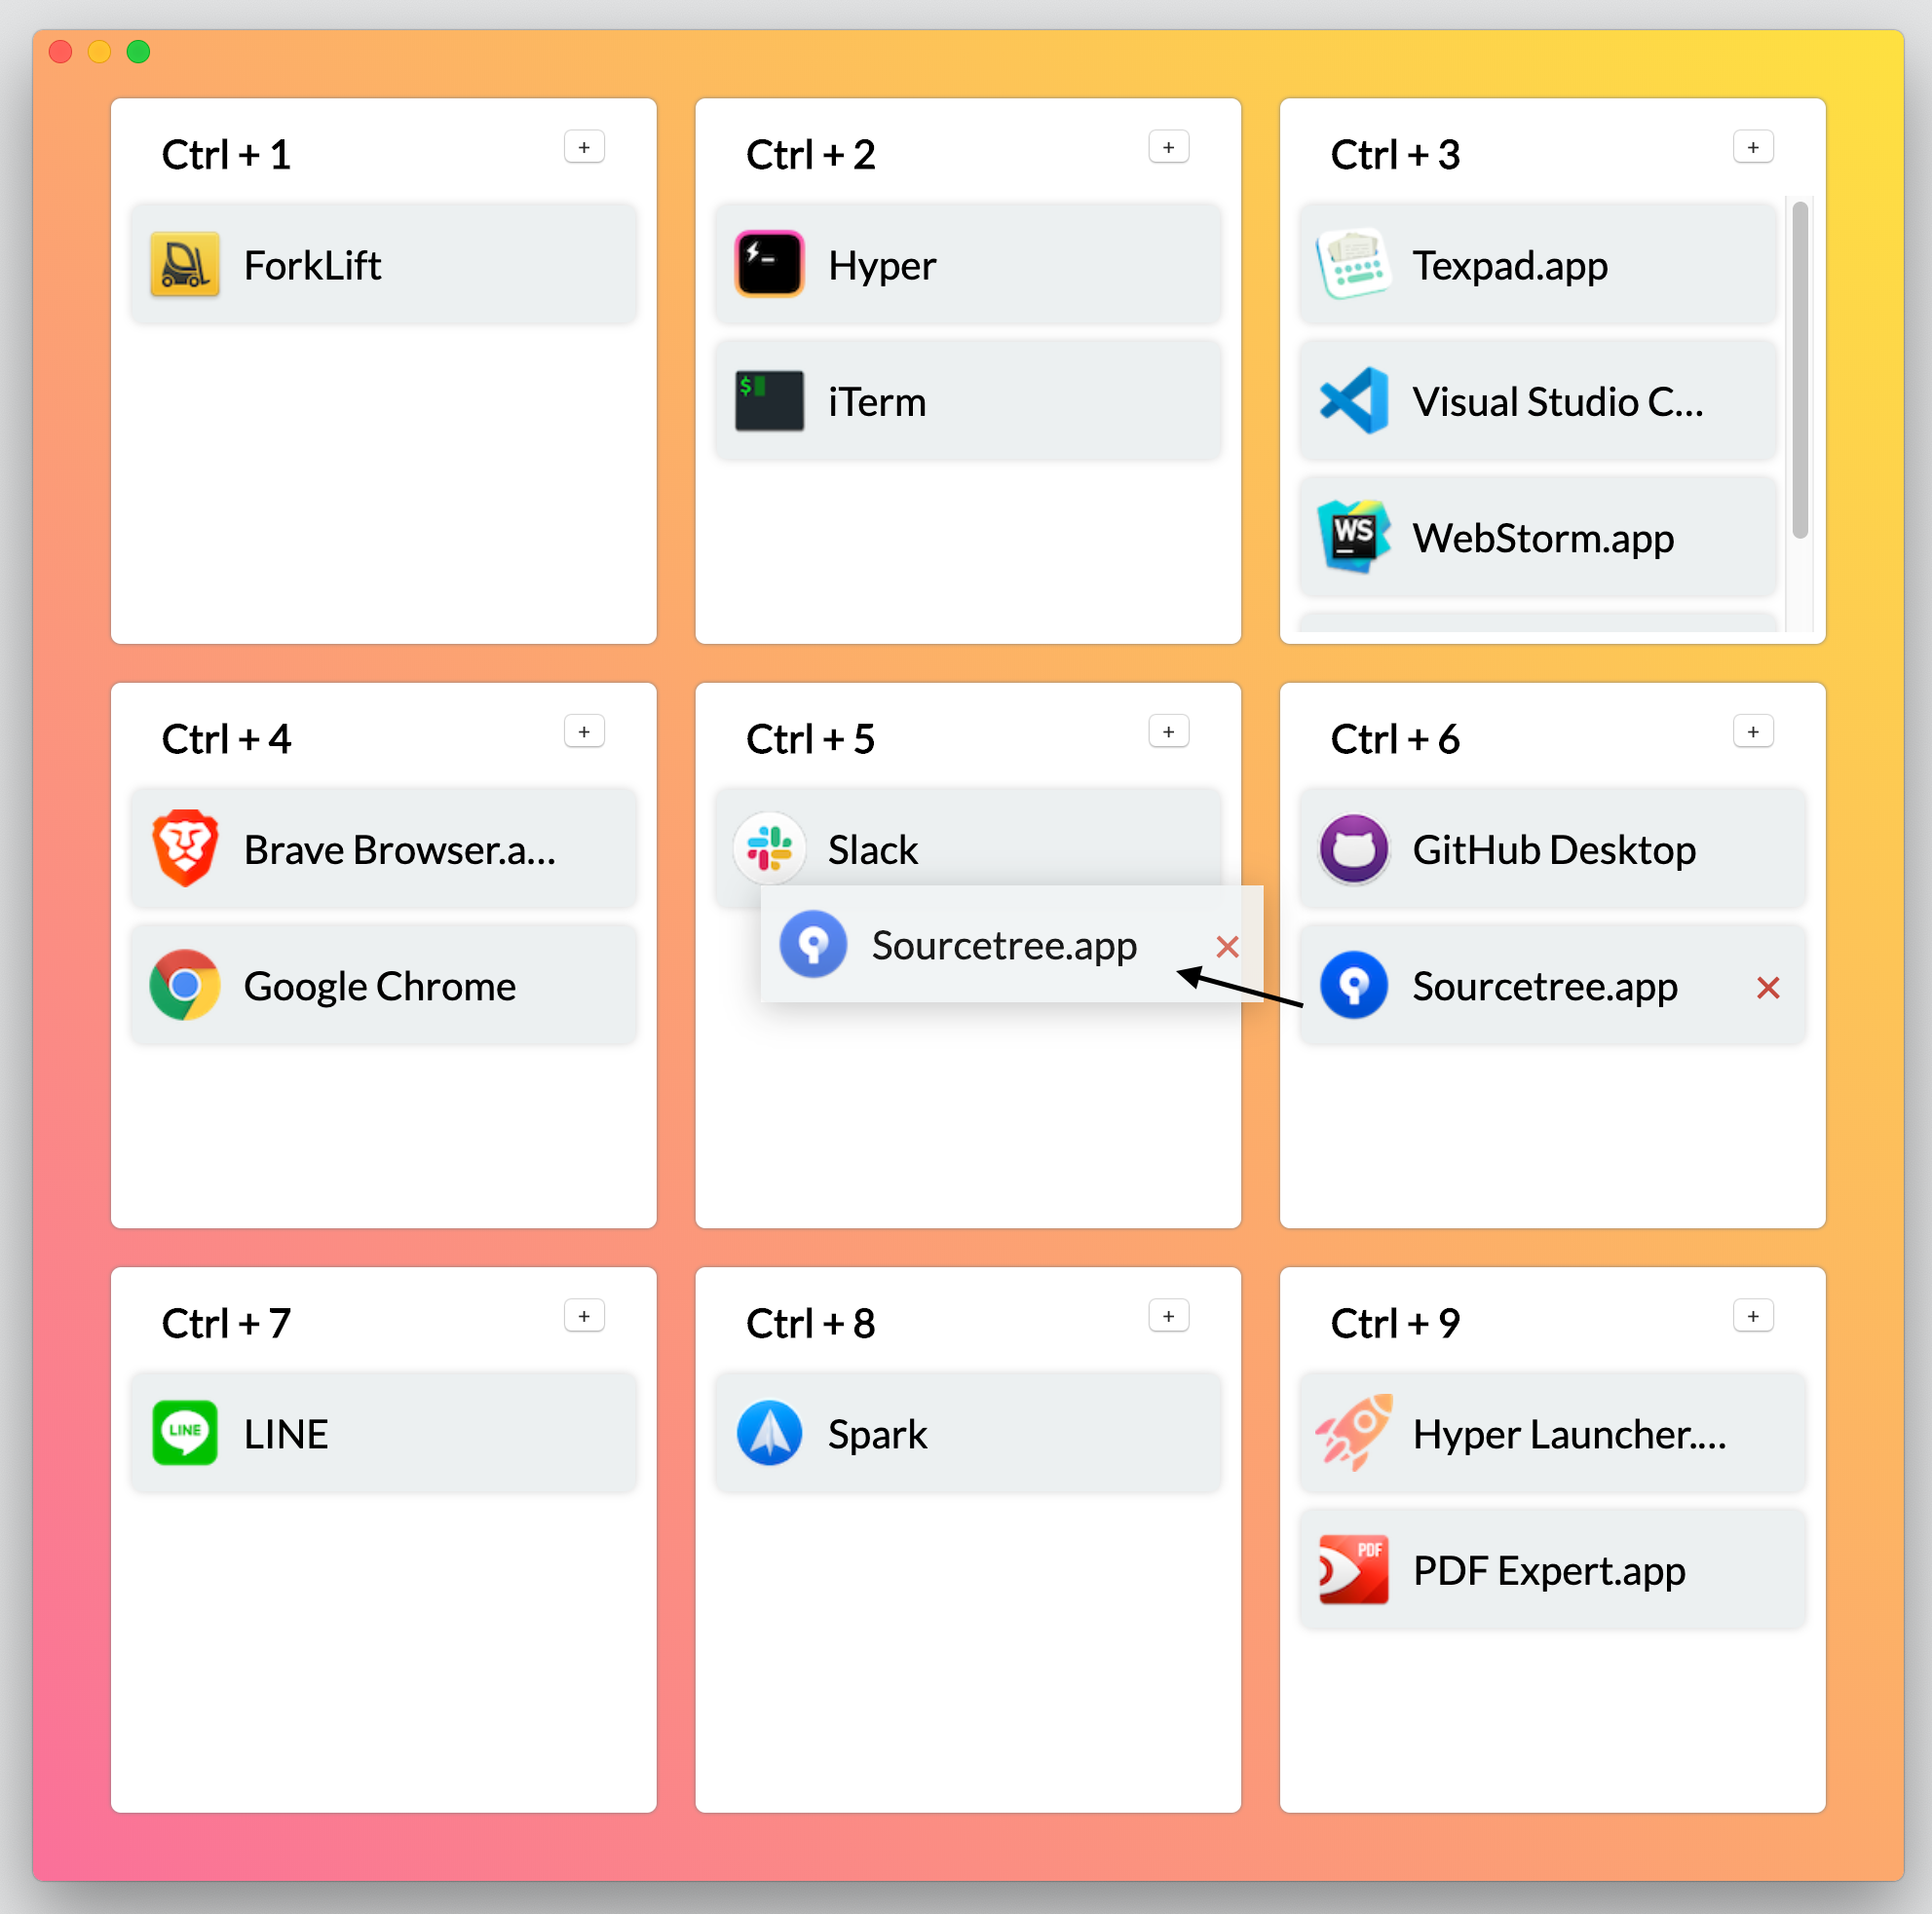
\includegraphics[width=100mm]{images/change}}
    \end{center}
    \caption{登録の変更}
    \label{fig:change}
\end{figure}

\begin{figure}[h]
    \begin{center}
       \fbox{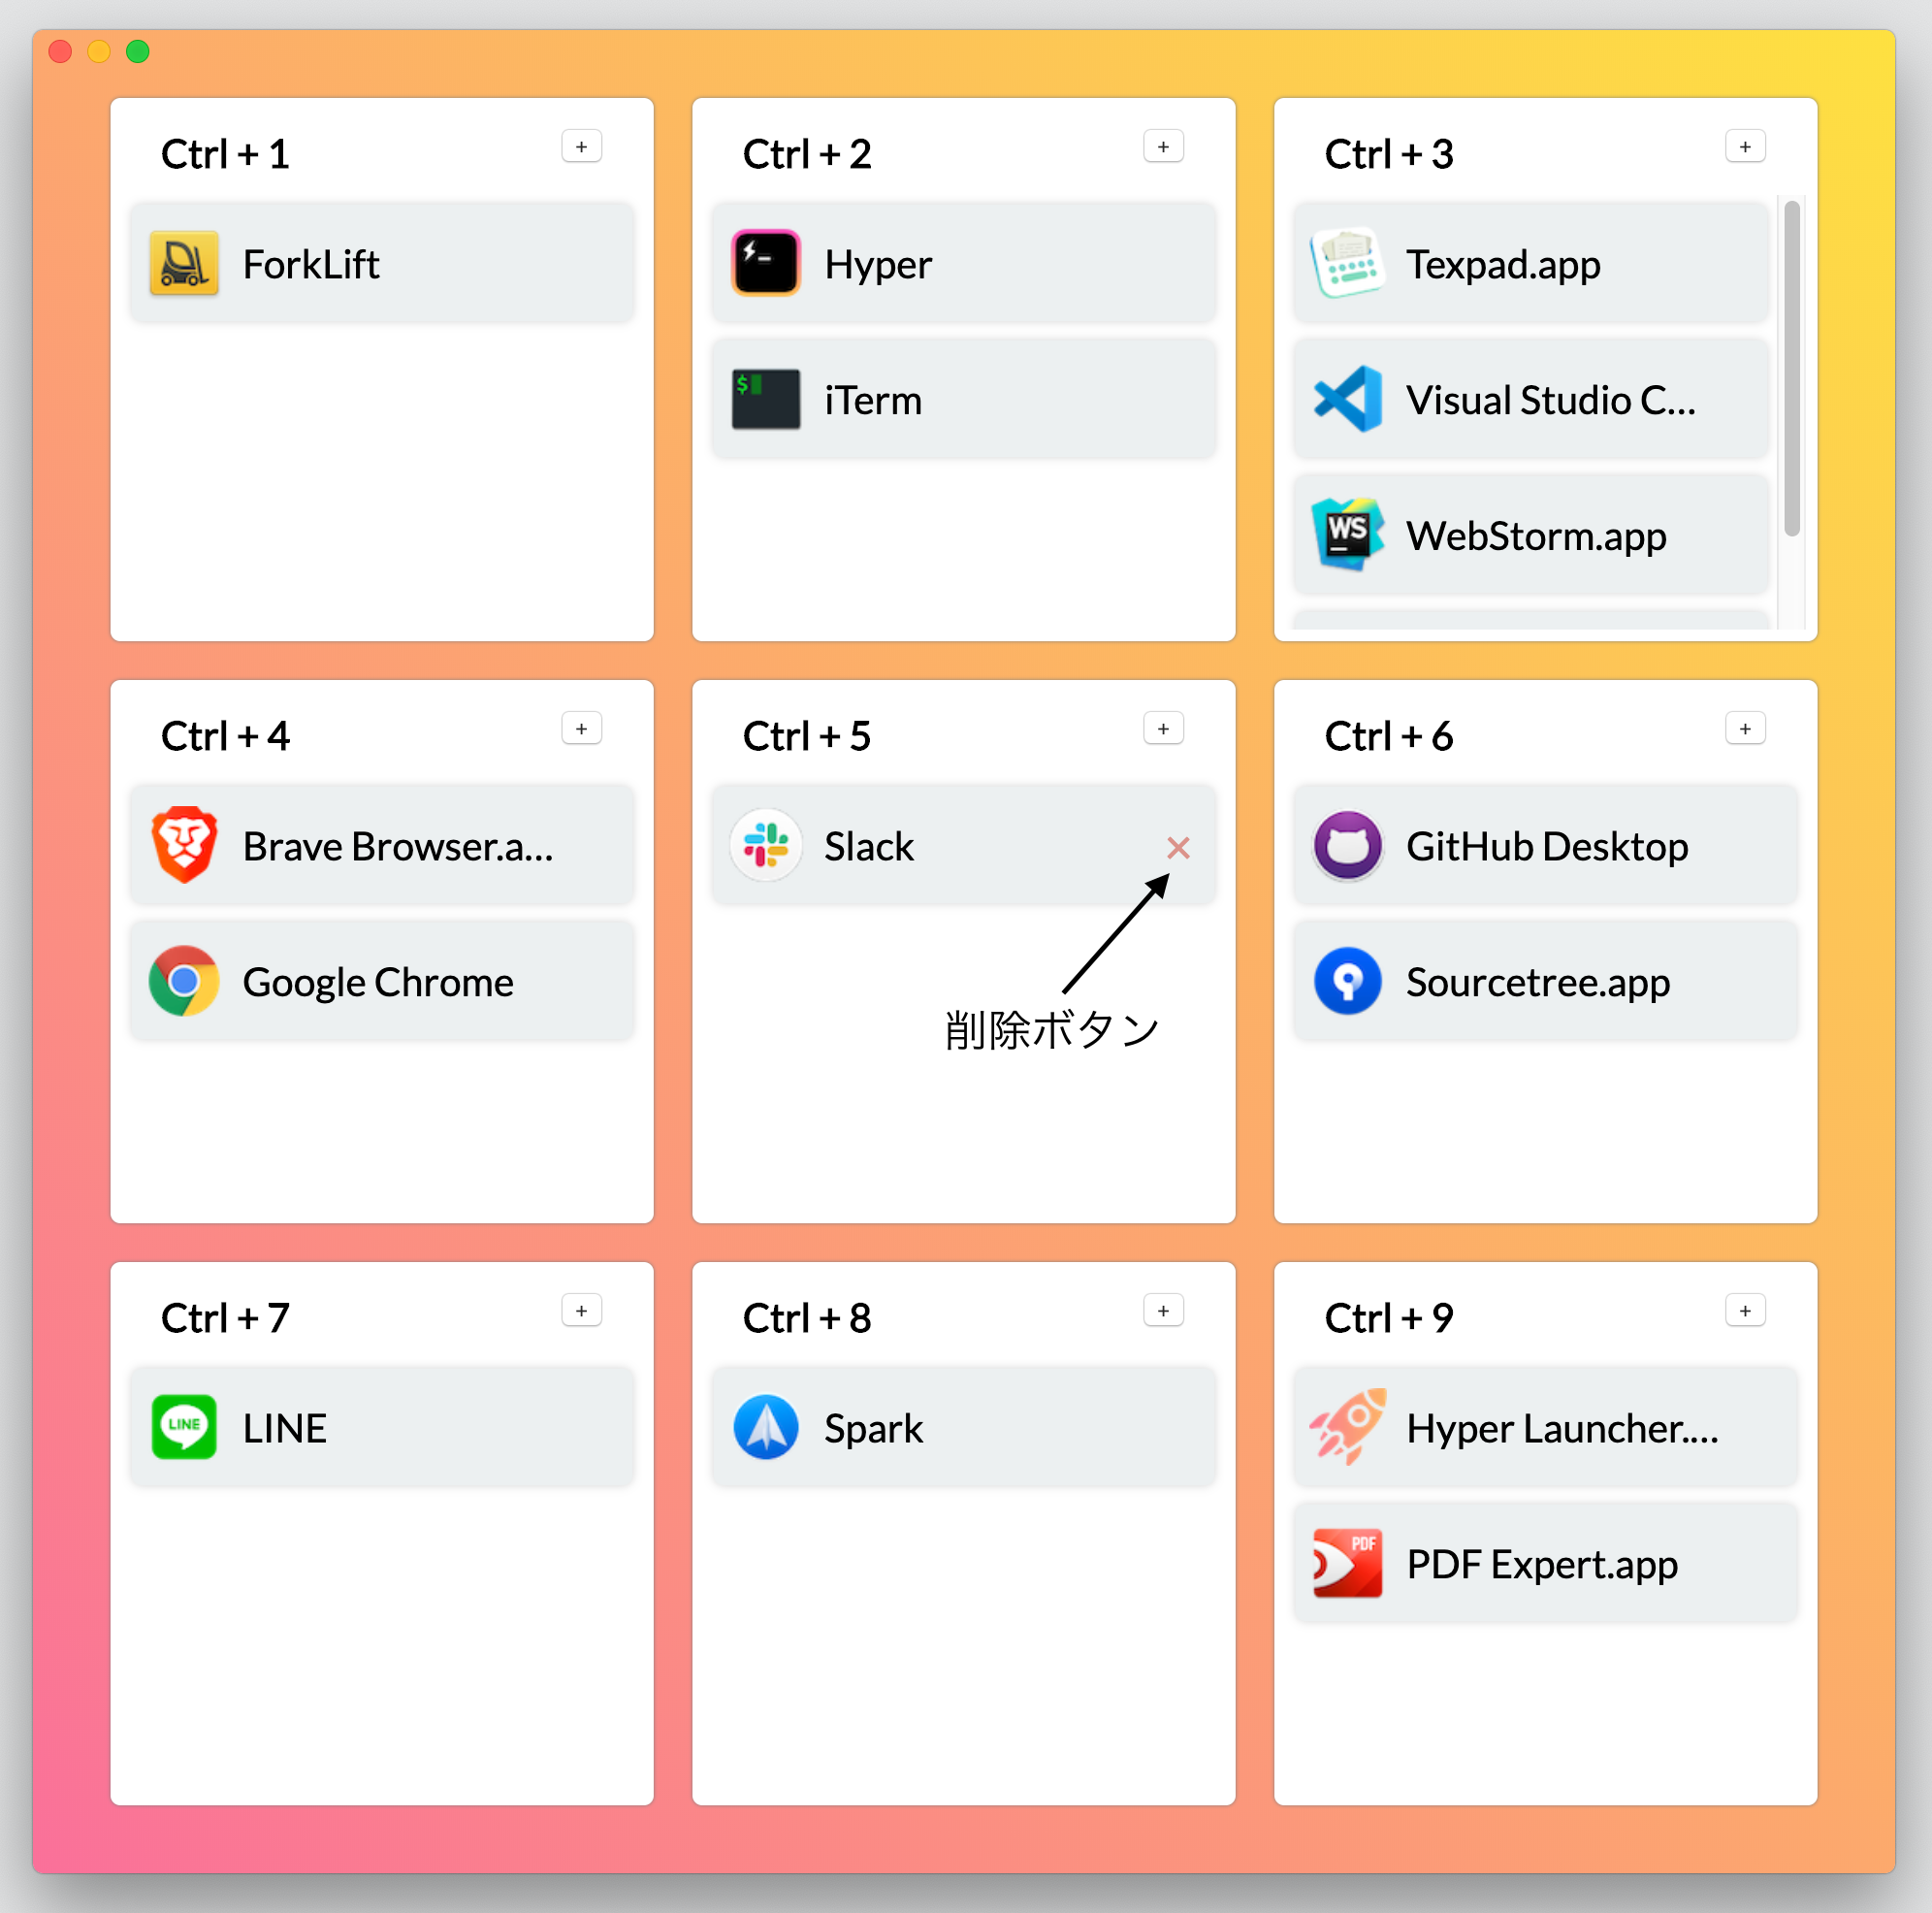
\includegraphics[width=100mm]{images/delete}}
    \end{center}
    \caption{登録の解除}
    \label{fig:delete}
\end{figure}

\subsection{複数登録と操作}
既にアプリケーションが登録されているセクションに、同じように新しいアプリケーションを追加するだけで複数のアプリケーションを登録することができる。アプリケーションは表示されている順番によって優先順位が定められており、キーを入力する度にその優先順位に基づき順番に起動するようになっている。その優先順についてもドラッグアンドドロップするだけで変更することができる。